\mode*

\section[Dokumentation]{Pythons dokumentation: string och list}

\begin{frame}
  \begin{block}{Strängar}
    \begin{itemize}
      \item Pythons dokumentation:
        \url{https://docs.python.org/3/library/stdtypes.html\#string-methods}
    \end{itemize}
  \end{block}

  \begin{exercise}[Strängar]
    \begin{itemize}
      \item Varje grupp svarar på en av frågorna
        \begin{enumerate}
          \item Vad har capitalize för parametrar och returvärden?
          \item Vad har count för parametrar och returvärden?
          \item Vad gör metoden split? Vilken datatyp returneras?
          \item Vad gör metoden strip?
        \end{enumerate}
      \item och konstruerar ett eget exempel för metoden.
    \end{itemize}
  \end{exercise}
\end{frame}

\begin{frame}
  \begin{block}{Listor}
    \begin{itemize}
      \item Pythons dokumentation
        \url{https://docs.python.org/3/tutorial/datastructures.html}
    \end{itemize}
  \end{block}

  \begin{exercise}[Listor]
    \begin{itemize}
      \item Varje grupp svarar på en av följande frågor:
        \begin{enumerate}
          \item Vad har append för parametrar och returvärden?
          \item Vad är skillnaden mellan append, extend och insert?
          \item Vad är skillnaden mellan remove och pop?
          \item Läs om copy. Vad menas med \enquote{shallow copy}?
        \end{enumerate}
      \item och konstruerar ett exempel för respektive metod.
    \end{itemize}
  \end{exercise}
\end{frame}

\begin{frame}
  \begin{question}
    \begin{itemize}
      \item Finns det någon metod här som inte har returvärde? Jämför med 
        strängmetoderna och förklara skillnaden.
    \end{itemize}
  \end{question}
\end{frame}


\section[Abstrakt datatyp]{Abstrakt datatyp för temperatur}

\begin{frame}
  \begin{block}{Temperatur}
    \begin{itemize}
      \item Temperatur kan anges i olika skalor.
      \item En abstrakt datatyp minskar risken för missförstånd.
    \end{itemize}
  \end{block}
  \begin{exercise}[Klass för temperatur]
    \begin{itemize}
      \item Konstruera en klass Temp som representerar en temperatur.
    \end{itemize}
    \begin{enumerate}
      \item Diskutera först vilka attribut och metoder som behövs, skriv sedan 
        koden.
        \pause
      \item Testa klassen i ett program som läser in utomhustemperaturen 
        (Celsius) och skriver ut temperaturen så att en amerikan förstår 
        (Fahrenheit).
    \end{enumerate}
  \end{exercise}
\end{frame}

\begin{frame}[fragile]
  \texttt{temp.py}\hrulefill
  \inputminted{python}{src/temp.py}
\end{frame}

\begin{frame}
  \begin{question}
    \begin{itemize}
      \item Vad är relationen mellan en klass och ett objekt?
      \item Om du skulle skriva dokumentation för klassen, vad är viktigt att 
        ta med?
    \end{itemize}
  \end{question}
\end{frame}


\section[Stack, länkad lista]{Stack implementerad med länkad lista}

\begin{frame}
  \begin{exercise}[Stack]
    \begin{itemize}
      \item Rita bilder som visar hur det ser ut när man lägger in ett nytt 
        element i stacken.
      \item Rita bilder som visar hur det ser ut när man tar bort ett element 
        från stacken.
      \item Rita bilder som visar en länkad lista.
    \end{itemize}
  \end{exercise}
\end{frame}

\begin{frame}
  \begin{figure}
    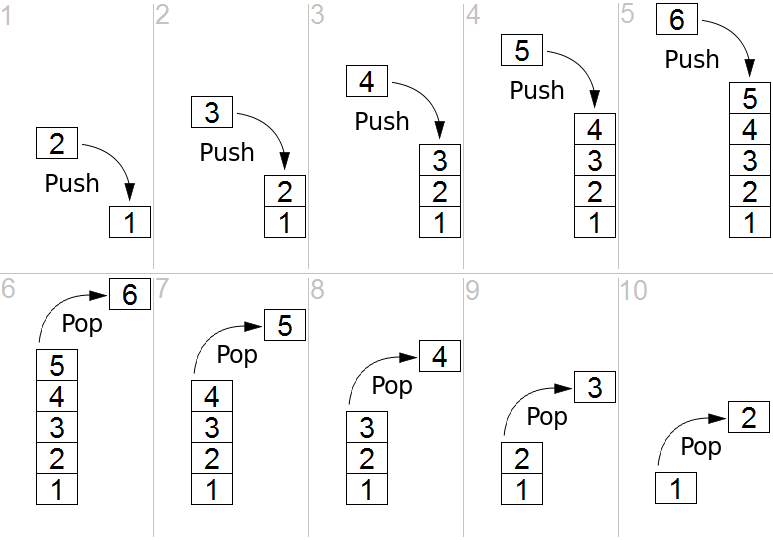
\includegraphics[height=0.8\textheight]{fig/lifo-stack.png}
    \caption{En stack, d.v.s.\ en sist-in-först-ut-kö.}
  \end{figure}
\end{frame}

\begin{frame}
  \begin{figure}
    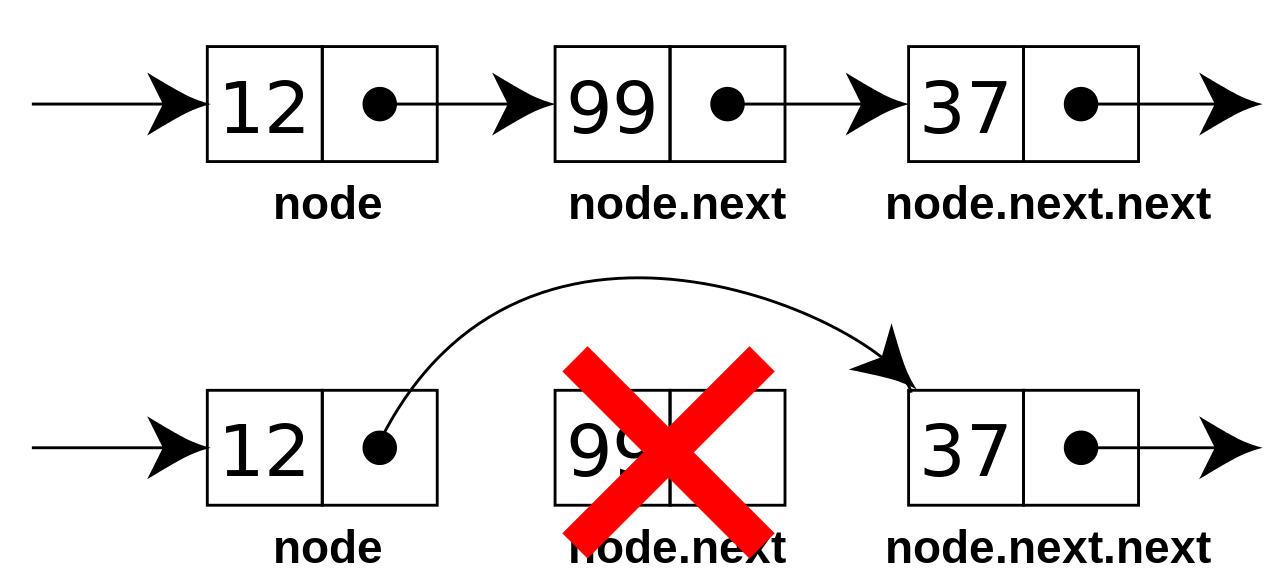
\includegraphics[width=\columnwidth]{fig/linked-list.png}
    \caption{En länkad lista.}
  \end{figure}
\end{frame}

\begin{frame}
  \begin{exercise}[Länkad lista]
    \begin{itemize}
      \item Skriv en klass för noder i en länkad lista.
      \item Skriv en klass för stackar med hjälp av nodeklassen.
    \end{itemize}
  \end{exercise}
\end{frame}

\begin{frame}[fragile]
  \texttt{stack.py}\hrulefill
  \inputminted{python}{src/stack.py}
\end{frame}


\section{Gamla tentafrågor}

\begin{frame}
  \begin{block}{Betygskriterier}
    \begin{itemize}
      \item[E]
        För betyg E ska man kunna avgöra vilken algoritm som löser ett givet 
        problem, kunna beskriva algoritmen och demonstrera den steg för steg 
        med givna data, samt implementera den. Motsvarande gäller för 
        datastrukturer.

        \pause

      \item[C]
        För betyg C ska kraven för betyg E vara uppfyllda, och dessutom ska man 
        kunna jämföra algoritmer och datastrukturer och bedöma dessas 
        lämplighet för ett givet problem. Här ställs också krav på 
        tidsplanering. Se tidsgränser för aktuell kursomgång under 
        Laborationer.

        \pause

      \item[A]
        För betyg A ska kraven för betyg C vara uppfyllda, och man ska dessutom 
        kunna modifiera/kombinera algoritmer och datastrukturer för att lösa 
        nya problem. Här ställs också höga krav på tydlighet i 
        algoritmbeskrivningar.
    \end{itemize}
  \end{block}
\end{frame}

\begin{frame}
  \begin{exercise}[E-nivå]
    \begin{quotation}
      Cyklisterna köar vid övergångsstället nere vid Valhallavägen. Först i kön 
      står Linda, sen Alexander, sen Robert och sist Marko.

      Kön är implementerad med en länkad lista. Rita bilder som visar hur det 
      ser ut i detalj (varje steg) när man sätter in respektive plockar ut ett 
      element ur kön.
    \end{quotation}
  \end{exercise}
\end{frame}

\begin{frame}
  \begin{exercise}[C-nivå]
    \begin{quotation}
      En norrskensentusiast vill lagra bilder på norrsken. Vad finns det för 
      fördelar respektive nackdelar med en vektor respektive en länkad lista 
      när det gäller
      \begin{itemize}
        \item åtkomst
        \item insättning
        \item borttagning
      \end{itemize}
      Svara med en tabell med tre rader.
    \end{quotation}
  \end{exercise}
\end{frame}

\begin{frame}
  \begin{exercise}[A-nivå]
    \begin{quotation}
      Våra datorer läser texter radvis, från vänster till höger. Men japansk 
      text står i kolumner uppifrån och ner, som läses från höger till vänster.

      Ge en algoritm för att med hjälp av en abstrakt kö eller stack ordna om 
      en japansk text om m kolumner och n rader.

      Exempel:
      \(\begin{matrix}
        7 & 4 & 1 \\
        8 & 5 & 2 \\
        9 & 6 & 3
      \end{matrix}\)
      läses in som 7 4 1 8 5 2 9 6 3, men vi vill ha ordningen 1 2 3 4 5 6 7 8 
      9.

      Du kan förutsätta att alla kolumner och rader är helt fyllda, men antalet 
      kolumner, m, behöver inte vara detsamma som antal rader, n. Till exempel 
      kan det finnas fem rader men bara tre kolumner.
      
      Visa sedan hur din algoritm fungerar för exemplet ovan.

      Utred till sist vilken komplexitet din algoritm har!
    \end{quotation}
  \end{exercise}
\end{frame}
